% Owner: Fatima Malik / Member B.
% Local font encoding restores the template's Times regular/bold faces under XeTeX.
\begingroup
\renewcommand{\encodingdefault}{T1}
\fontencoding{T1}\selectfont
\chapter{Proposed Approach and Methodology}
Zeest uses an integration methodology rather than a new diagnostic algorithm. The method begins with a physician-selected patient and encounter, then prepares consultation notes, clinical inputs and relevant longitudinal history. Existing imaging models, clinical language-model capability and retrieval methods act as supporting components, while the project contribution is the way their outputs connect to patient memory, evidence and physician approval. Chapter~4 defines the workflow for navigation, transcription, input handling, memory retrieval, draft generation, critic review and revision-specific decisions. This chapter turns those requirements into a controlled research procedure in which each stage keeps patient, encounter and source context visible, so a generated draft can be inspected rather than treated as final. The methodology is organised around three questions: how the current encounter and history should be prepared for specialised agents, how external evidence should be retrieved and attached to the draft for physician review, and how variants should be compared so memory, agent decomposition, critic review and multimodal inputs can be assessed. The answers are expressed as a processing pipeline, dataset and model register, evidence-retrieval procedure and ablation protocol.

\section{Case Preparation and Input Handling}
The first methodological step is to create a consistent case package for the selected encounter. The physician opens a patient record, reviews prior encounters and begins or uploads consultation information according to the workflow defined in Chapter~4. Consultation audio is prepared as structured notes, which the physician can inspect and correct before downstream use. Imaging, laboratory information and medication context remain separate because they have different representations, source formats and analysis needs. Each input must retain its patient identifier, encounter identifier, type, source reference and revision. This prevents later stages from mixing old notes with the current encounter or treating unsupported input as a finding. The prepared package therefore describes what information is available, where it came from and whether it is ready for analysis. This also keeps failed or missing inputs visible instead of hiding them inside the draft generation process. The purpose of this stage is not to diagnose the patient, but to create a clear and traceable input state for memory retrieval, specialist analysis and later comparison.

\section{Hybrid Memory and Case Organisation}
Hybrid memory connects the current encounter to relevant historical context. Relational records preserve patient, encounter, input and approved-decision relationships, while semantic retrieval selects history related to the current consultation or clinical question. The Patient Memory Agent returns source-aware context, not a final diagnosis. The Clinical Case Agent then organises corrected notes, retrieved history and specialist inputs into a case representation for later reasoning. This package identifies what is current, what is historical, what was retrieved and what is missing. If an input is absent or fails validation, that status is carried forward instead of creating a placeholder finding. This approach aligns with the database design in Chapter~4, where clinical inputs, drafts, evidence, audit actions and approved decisions are separate records. It also supports the planned comparison with a single-LLM baseline, because the baseline receives less patient-specific structure than the memory and full-system variants. The case organisation stage is therefore the bridge between raw encounter information and the controlled agent workflow.

\section{Proposed Agent Processing Pipeline}
Figure~\ref{fig:fatima:method-pipeline} shows the processing pipeline used to coordinate the proposed Zeest workflow. The physician-facing interface produces current case inputs, while hybrid memory supplies patient history. The Clinical Case Agent combines those inputs and sends modality-specific information to the Imaging, Laboratory and Medication Safety agents. The Imaging Agent uses an existing validated pre-trained model only for supported imaging tasks. The Laboratory Agent analyses supplied laboratory information, and the Medication Safety Agent checks medication context against a resource still to be selected. The Evidence and RAG Agent retrieves external clinical material with source references. The Clinical Reasoning Agent drafts the diagnosis and treatment proposal, and the Safety and Critic Agent checks it before physician review. The pipeline separates data movement from decision authority. Agents may prepare, analyse, retrieve or review information, but they do not record a final clinical decision. The physician sees the draft with evidence and critic findings, then approves, modifies or rejects it. Approval records the accepted revision, modification creates a changed draft, and rejection keeps the draft out of approved decisions.

\begin{figure}[htbp]
\centering
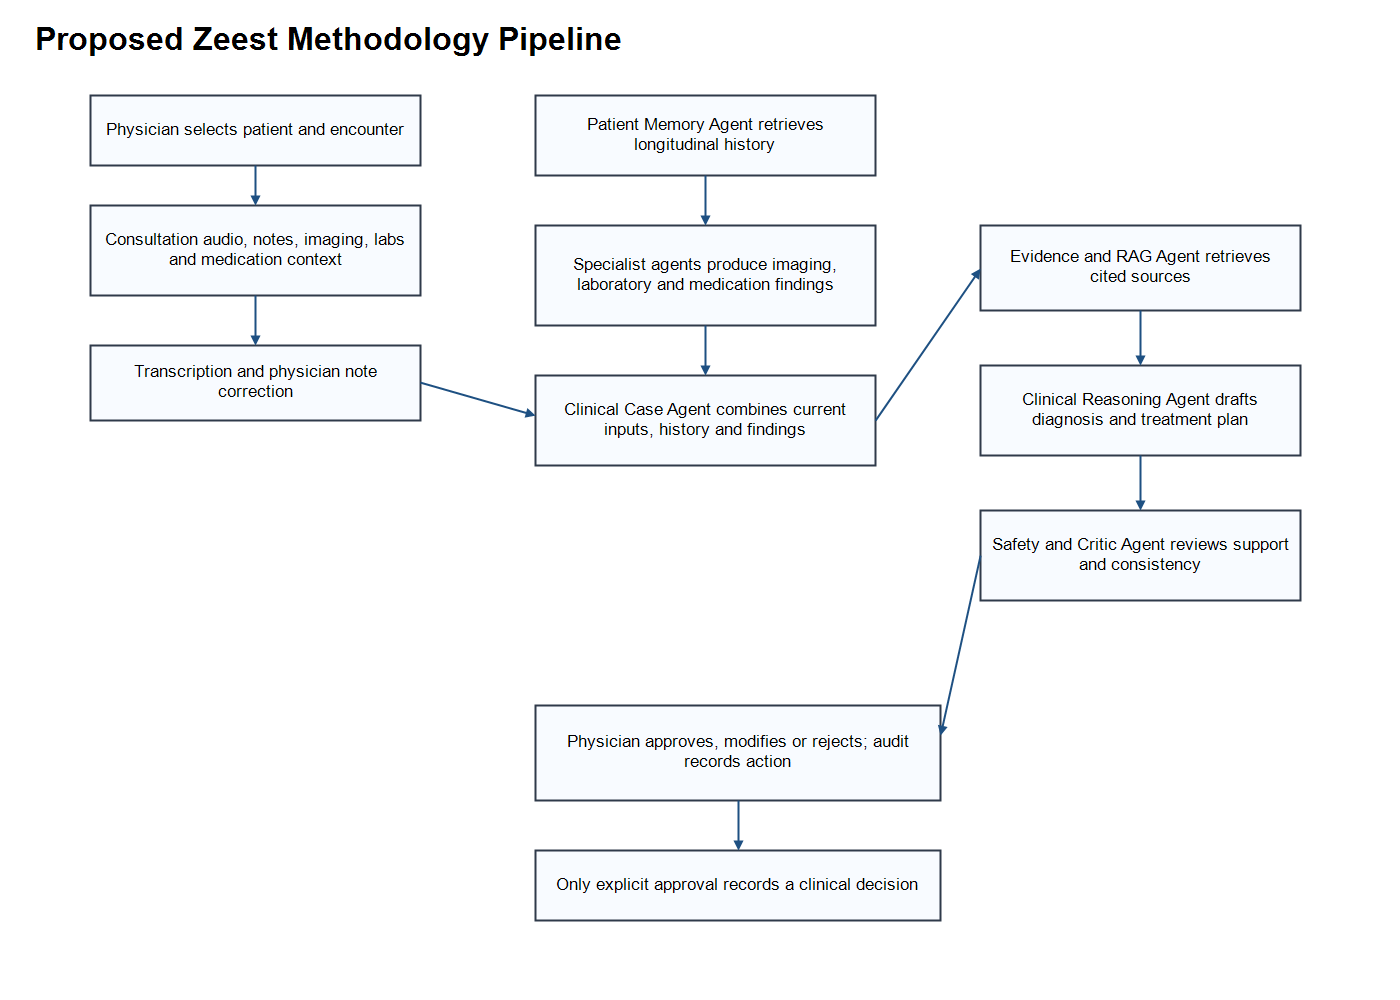
\includegraphics[width=0.96\textwidth,height=0.78\textheight,keepaspectratio]{Figures/fatima_D04_method_pipeline.png}
\caption{Proposed Zeest methodology pipeline connecting consultation inputs, hybrid memory, specialist agents, evidence retrieval, clinical drafting, critic review and physician decision controls.}
\label{fig:fatima:method-pipeline}
\end{figure}

\section{Dataset, Model and Resource Register}
The candidate data and model resources come from the proposal and literature review. MIMIC-IV supports de-identified longitudinal EHR cases, while MIMIC-CXR and CheXpert support chest radiograph tasks. PubMed or guideline sources may support evidence retrieval, and Synthea can support synthetic patient cases.\cite{zeestA:mimicIV,zeestB:mimiccxr,zeestB:chexpert,zeestB:synthea} These resources are not interchangeable. Longitudinal memory needs encounter context, while imaging cases must match the selected model's supported labels. Evidence retrieval needs a permitted corpus and citation preservation. Medication review requires a knowledge resource with suitable coverage, and semantic memory requires an embedding model compatible with the vector store. Table~\ref{tab:fatima:dataset-register} records each candidate's role, status and unresolved dependency so final selection is not assumed before implementation. This register keeps the methodology honest: a proposal-listed resource becomes usable only after access, permitted use, preprocessing needs and clinical-domain fit are confirmed. It also gives later evaluation work a checklist for deciding which cases and modalities can be included in the ablation study.

\begin{table}[htbp]
\centering
\scriptsize
\caption{Proposed dataset, model and resource register for Zeest methodology.}
\label{tab:fatima:dataset-register}
\begin{tabular}{|p{0.19\textwidth}|p{0.24\textwidth}|p{0.21\textwidth}|p{0.22\textwidth}|}
\hline
Candidate & Planned role & Current status & Dependency \\ \hline
MIMIC-IV \cite{zeestA:mimicIV} & Longitudinal EHR-style case context. & Candidate source. & Access, permitted use and case selection. \\ \hline
MIMIC-CXR \cite{zeestB:mimiccxr} & Chest radiograph and report context. & Candidate source. & Access, pairing and supported task. \\ \hline
CheXpert \cite{zeestB:chexpert} & Imaging benchmark/model candidate domain. & Candidate source. & Final model and label compatibility. \\ \hline
Existing imaging classifier & Supported imaging finding generation. & Not selected. & Validated model, inputs and labels. \\ \hline
PubMed/guideline corpus & External evidence retrieval. & Not finalised. & Corpus choice, citation format and retrieval policy. \\ \hline
Synthea \cite{zeestB:synthea} & Synthetic workflow cases. & Candidate source. & Scenario realism and mapping to Zeest fields. \\ \hline
Medication knowledge resource & Medication safety checking. & Not selected. & Resource availability and interaction coverage. \\ \hline
Embedding model & Semantic memory and retrieval. & Not selected. & Dimension, domain suitability and pgvector storage. \\ \hline
\end{tabular}
\end{table}

\section{Data Preprocessing}
Preprocessing depends on the chosen resources, but Zeest's workflow already defines the preparation rules. Patient and encounter identifiers must be de-identified or synthetic. Consultation notes, reports and other text inputs should be structured while remaining linked to their source. Imaging files should follow only the selected model's required input format, because changing image preparation without matching the model can invalidate the finding. Laboratory and medication information should be normalised enough for the relevant agent to interpret it, but missing values should not be invented. Evidence passages should retain source references and retrieval timestamps. Ablation cases should be frozen before comparison so each variant receives the same allowed inputs for its configuration. This prevents a memory-augmented variant or full-system variant from benefiting from accidental case changes. The preprocessing stage therefore supports both system correctness and evaluation fairness. It prepares the data for analysis while preserving the traceability needed for physician review, critic checking and later reporting.

\section{Evidence Retrieval Method}
The evidence method separates patient-specific context from external clinical knowledge. Patient context comes from the selected encounter, corrected notes, retrieved history and specialist findings. External knowledge comes from guideline, literature or medical reference material selected for retrieval. The Evidence and RAG Agent forms a query from the case context, retrieves candidate passages, filters or ranks them by relevance and returns supporting text with citations. Figure~\ref{fig:fatima:evidence-retrieval} shows this flow. The Clinical Reasoning Agent may use retrieved evidence when drafting a diagnosis and treatment plan, but the evidence must remain visible to the physician. This prevents a black box answer and lets the critic identify unsupported claims, missing evidence or contradictions. The procedure also supports traceability because a draft should identify which retrieved passages were used and where they came from. The physician can then judge whether the support fits the current patient and whether the draft should be approved, edited or rejected. If evidence is insufficient, the interface should show that status instead of fabricating support.

\begin{figure}[htbp]
\centering
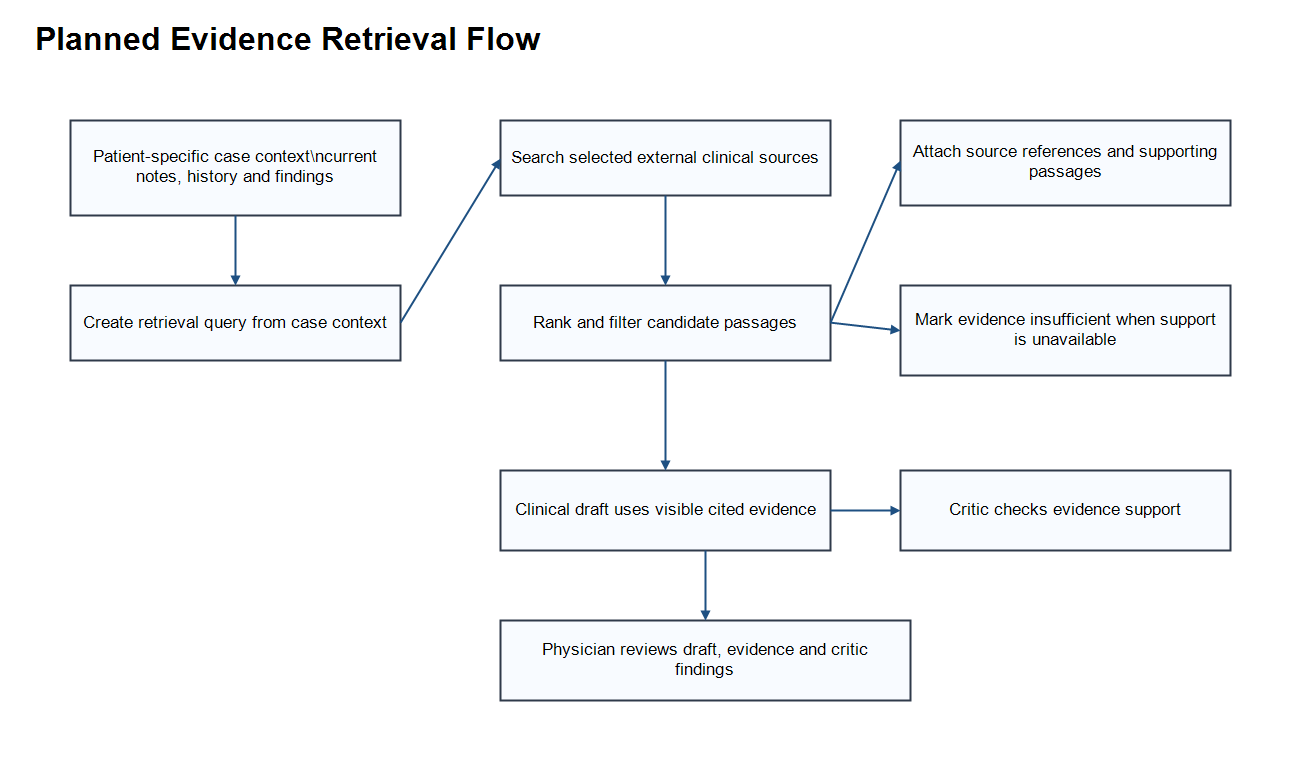
\includegraphics[width=0.92\textwidth,height=0.62\textheight,keepaspectratio]{Figures/fatima_D06_evidence_retrieval.png}
\caption{Planned evidence retrieval procedure separating patient-specific case context from external clinical sources before cited passages are attached to the clinical draft.}
\label{fig:fatima:evidence-retrieval}
\end{figure}

\section{Ablation and Evaluation Protocol}
The ablation protocol answers Zeest's evaluation questions. The comparison includes a single LLM baseline, a memory-augmented variant and the full Zeest system. The baseline receives the current case prompt only. The memory variant adds retrieved patient history, while the full system adds specialist findings, evidence retrieval and critic review. Figure~\ref{fig:fatima:ablation-protocol} shows how the same case set flows through the variants and into one assessment process. Additional contrasts examine critic and multimodal contribution where the selected cases support them. The same reference judgement process must be used for every variant. Table~\ref{tab:fatima:experiment-protocol} defines the variants and comparison controls. Outputs should be assessed for case relevance, patient-history use, evidence support, consistency with specialist findings, critic handling and physician reviewability. Metrics, sample counts, rubrics and reviewer roles remain unresolved. Possible measures include agreement with a reference judgement, citation relevance, unsupported-claim count, error categories and physician review effort. Each run should retain its configuration and output, and cases should not change between variants except for intentionally withheld inputs.

\begin{figure}[htbp]
\centering
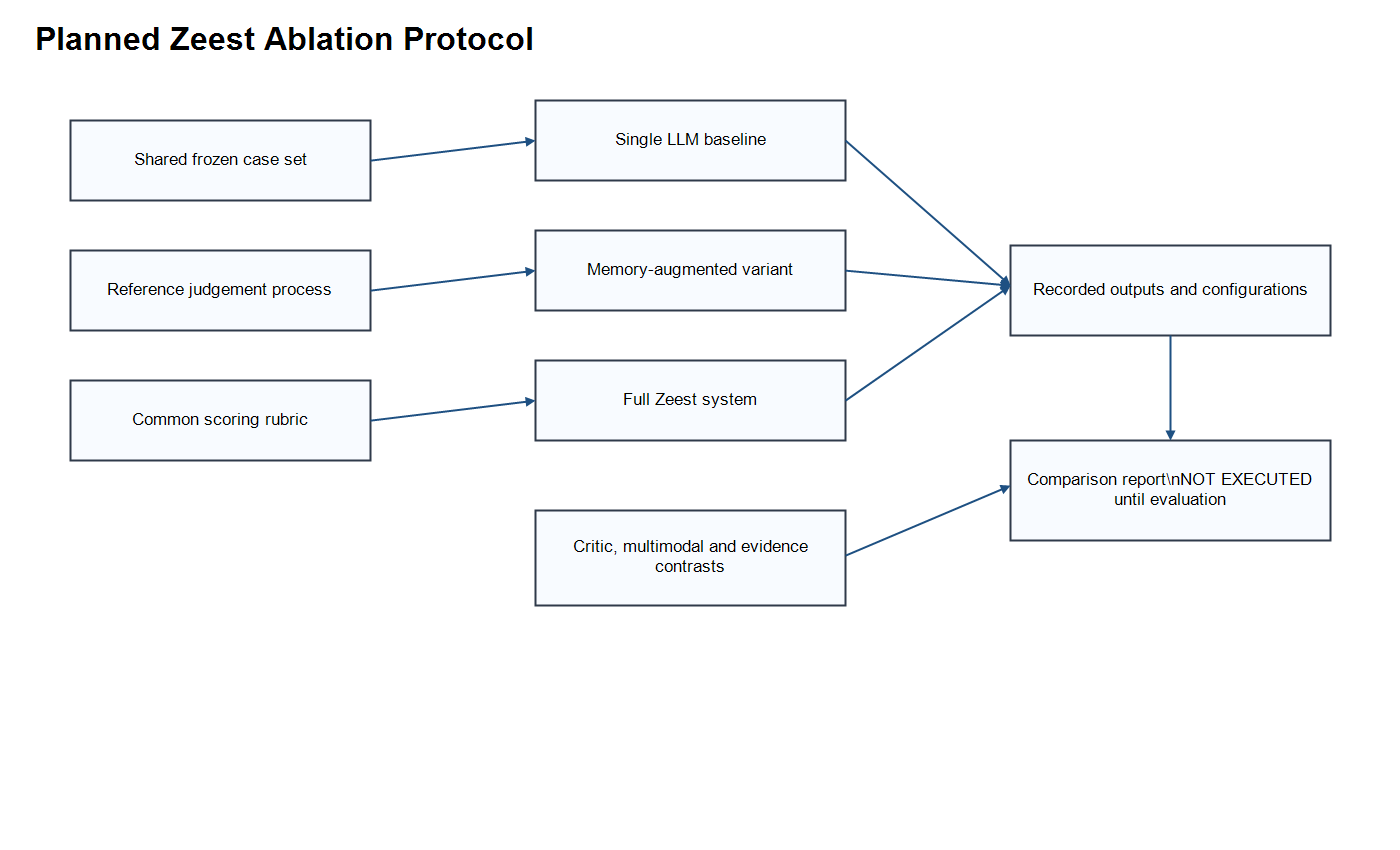
\includegraphics[width=0.96\textwidth,height=0.66\textheight,keepaspectratio]{Figures/fatima_D05_ablation_protocol.png}
\caption{Planned ablation protocol comparing a single LLM baseline, memory-augmented variant and full Zeest system using shared cases and a common reference assessment process.}
\label{fig:fatima:ablation-protocol}
\end{figure}

\begin{table}[htbp]
\centering
\scriptsize
\caption{Planned ablation and evaluation protocol for Zeest variants.}
\label{tab:fatima:experiment-protocol}
\begin{tabular}{|p{0.19\textwidth}|p{0.27\textwidth}|p{0.21\textwidth}|p{0.19\textwidth}|}
\hline
Variant or contrast & Inputs allowed & Planned assessment focus & Status \\ \hline
Single LLM baseline & Current case prompt only. & Draft relevance and unsupported claims. & Not executed. \\ \hline
Memory-augmented & Current case plus retrieved longitudinal history. & Contribution of patient memory. & Not executed. \\ \hline
Full Zeest & Case, memory, specialist findings, evidence and critic review. & Integrated workflow performance and reviewability. & Not executed. \\ \hline
Critic contrast & Full pipeline with and without critic findings. & Unsupported or contradictory output handling. & Planned control. \\ \hline
Multimodal contrast & Text-only case versus supported multimodal case. & Contribution of imaging/lab/medication findings. & Planned control. \\ \hline
Evidence contrast & Draft with and without retrieved cited passages. & Citation support and evidence relevance. & Planned control. \\ \hline
\end{tabular}
\end{table}

\section{Methodological Traceability}
The proposed methodology traces to the objectives and requirements in Chapters~2 and~4. Hybrid memory supports O1, FR18 and FR19. Transcription and note correction support O2 and FR09 through FR13. Specialist agents support O3 and FR20 through FR25. Imaging integration supports O4 and FR21, while evidence retrieval supports O5, FR27 and FR31. Clinical draft generation supports O6, FR28 and FR29. Critic review supports O7, FR30 and FR32. Physician approval, modification, rejection and audit support O8 and FR33 through FR38. The ablation protocol supports O9 and RR01 through RR04. Table~\ref{tab:fatima:method-trace} summarises this mapping so later design and evaluation work can remain aligned with the current requirements. This traceability matters because the methodology should evaluate the same workflow described in the requirements, not a different or simplified system. Later changes to IDs, selected datasets or agent responsibilities should therefore be reflected here and in Fatima's handoff before the report is considered final.

\begin{table}[htbp]
\centering
\small
\caption{Traceability between methodology stages and current requirement areas.}
\label{tab:fatima:method-trace}
\begin{tabular}{|p{0.24\textwidth}|p{0.28\textwidth}|p{0.34\textwidth}|}
\hline
Method stage & Related Chapter 4 IDs & Planned verification \\ \hline
Case preparation & FR04--FR17 & Check patient, encounter and source associations. \\ \hline
Hybrid memory retrieval & FR18--FR20 & Compare retrieved history against selected cases. \\ \hline
Specialist analysis & FR21--FR25 & Check input-specific findings and failures. \\ \hline
Evidence retrieval & FR27, FR31 & Assess citation relevance and passage support. \\ \hline
Clinical draft and critic & FR28--FR32 & Review draft consistency and critic findings. \\ \hline
Physician decision workflow & FR33--FR38 & Verify revision-specific approval and audit records. \\ \hline
Ablation framework & RR01--RR04 & Compare variants using shared cases and rubric. \\ \hline
\end{tabular}
\end{table}

\section{Dependencies and Open Method Decisions}
The methodology has unresolved dependencies before implementation and evaluation. The clinical domain must match available data, permitted use and an existing validated model. The transcription component, embedding model, evidence corpus, medication resource and LLM configuration remain to be selected. The LangGraph and Google ADK responsibility split remains a Chapter~6 design decision. Evaluation also needs reference judgements, reviewer roles, sample size, rubric and thresholds. These dependencies are important because they determine whether a case can be used, which modalities can be compared and how outputs should be judged. They also prevent the report from presenting design assumptions as completed results. This chapter therefore provides a structured plan without pretending those choices are complete. The open decisions should be closed before implementation claims or numerical evaluation results are added to the report, and any selected resource should be recorded with its permitted use and limitations. Keeping these items visible helps the team coordinate later design, testing and writing work.

\section{Conclusion}
In conclusion, Zeest's methodology combines case preparation, hybrid memory retrieval, specialist analysis, evidence-grounded drafting, critic review and physician decision control. It supports an R\&D investigation of whether memory, multimodal inputs, agent decomposition, evidence retrieval and critic review improve clinical draft reviewability. The figures and tables define input flow, unresolved resources and ablation comparisons. The procedure keeps the generated output as a draft until the physician approves, modifies or rejects it, preserving the approval boundary established in the requirements. Because the prototype is unbuilt, the chapter separates procedure from outcomes. Future work must confirm resources, implement the pipeline, execute comparisons and report measured findings with limitations. This structure gives the team a method for moving from the proposal and requirements toward a testable system while avoiding unsupported claims about clinical performance, dataset access or completed integration. It also helps later chapters and reviews check whether the design remains consistent with the planned evaluation.

\endgroup
